\documentclass[10pt,twocolumn]{article}
\usepackage[margin=0.72in]{geometry}
\usepackage{amsmath,amssymb,amsthm}
\usepackage{booktabs}
\usepackage{graphicx}
\usepackage{xcolor}
\usepackage{hyperref}
\usepackage{enumitem}

\hypersetup{
  colorlinks=true,
  linkcolor=blue!60!black,
  citecolor=blue!60!black,
  urlcolor=blue!60!black
}

\newtheorem{theorem}{Theorem}[section]
\newtheorem{lemma}[theorem]{Lemma}
\newtheorem{proposition}[theorem]{Proposition}
\newtheorem{corollary}[theorem]{Corollary}
\theoremstyle{definition}
\newtheorem{definition}[theorem]{Definition}
\newtheorem{remark}[theorem]{Remark}

\title{\textbf{Kernel-Checked Formalizations of Recently Settled Combinatorial\\
and Algebraic Problems in Lean~4:\\
Erd\H{o}s Problems 348, 216, 609, and Kourovka Counterexamples}}

\author{Mike Helsel\\
\small \texttt{ctrl} Formal Mathematics Laboratory}
\date{October 19, 2026}

\begin{document}
\maketitle

\begin{abstract}
We report a collection of complete, kernel-checked Lean~4 / Mathlib formalizations of recently resolved problems and classical theorems across additive combinatorics, discrete geometry, Ramsey graph theory, and group theory. Every formalization compiles with \textbf{zero \texttt{sorry}}, \textbf{zero \texttt{native\_decide}}, and depends strictly on the three standard foundational axioms (\texttt{propext}, \texttt{Classical.choice}, \texttt{Quot.sound}), with statement fidelity verified against \texttt{google-deepmind/formal-conjectures} and \texttt{lake comparator}. Our primary contributions encompass:
(1)~\textbf{Erd\H{o}s Problem~348} (\texttt{erdos-348-lean}, 1,180 LOC): a complete formalization of Geneson's 2026 deletion-threshold classification for complete sequences (\texttt{arXiv:2609.25107}), proving that a monotone sequence of natural numbers remains complete after deleting any $m$ terms but fails completeness after deleting any $n > m$ terms if and only if $m \le 1$;
(2)~\textbf{Erd\H{o}s Problem~216 for $k \ge 7$} (\texttt{lean-erdos-proofs/Solution.lean}, 965 LOC): a complete Euclidean formalization of Horton's theorem (1983), constructing arbitrarily large planar point sets in general position containing no empty convex $k$-gon for all $k \ge 7$;
(3)~\textbf{Erd\H{o}s Problem~609 at $n=3$} (\texttt{Erdos609.lean}, 410 LOC): a kernel-checked proof of Cai's $f(3)=5$ result on monochromatic odd cycles in 3-colorings of $K_9$;
(4)~\textbf{Kourovka Notebook \& MathOverflow Resolutions}: kernel-checked solutions to Kourovka Problems~17.32 (Ionin--Semidetnov 2026) and~19.35 (Bergman--McCulloch 2026), together with MathOverflow Problems 513215, 509929, 515611, and 501066; and
(5)~\textbf{Six Erd\H{o}s Variant Theorems in \texttt{ctrl/lean/ErdosLab}}: machine-checked proofs for Erd\H{o}s Problems~273 ($p \ge 3$), 292 ($\ge 2$ summands), 318 (single-even shift), 834 (3-uniform Li hypergraph), 885 ($k=3$), and 939 (infinite $r=6$ coprime 6-powerful triples).
\end{abstract}

\section{Introduction}

As mathematical research increasingly pairs human proofs with AI-assisted theorem proving, a central methodological challenge is \emph{statement fidelity}: ensuring that a formal proof checks the exact statement intended by the mathematical community without weakened definitions, smuggled axioms, or trusted external oracle reductions (\texttt{native\_decide}).

To enforce end-to-end trust, our formalization pipeline uses a strict \textbf{Challenge--Solution--Comparator} architecture:
\begin{enumerate}[leftmargin=1.4em,itemsep=2pt]
  \item \textbf{Immutable Challenge Specification}: Statement definitions are copied verbatim from \texttt{google-deepmind/formal-conjectures}~\cite{FormalConjectures} into a read-only \texttt{Challenge} module.
  \item \textbf{Kernel-Pure Solution}: The proof is developed in a separate module where \texttt{sorry}, \texttt{admit}, custom \texttt{axiom}/\texttt{opaque}, \texttt{implemented\_by}, \texttt{extern}, and \texttt{native\_decide} are mechanically banned; finite searches must use kernel-reduced \texttt{decide} (\texttt{decide +kernel}).
  \item \textbf{Comparator \& Axiom Audit}: Both modules are replayed through \texttt{lake comparator} (and \texttt{ctrl check}), verifying definitionally identical types and confirming that \texttt{\#print axioms} emits only \texttt{\{propext, Classical.choice, Quot.sound\}}.
\end{enumerate}

\begin{figure*}[t]
\centering
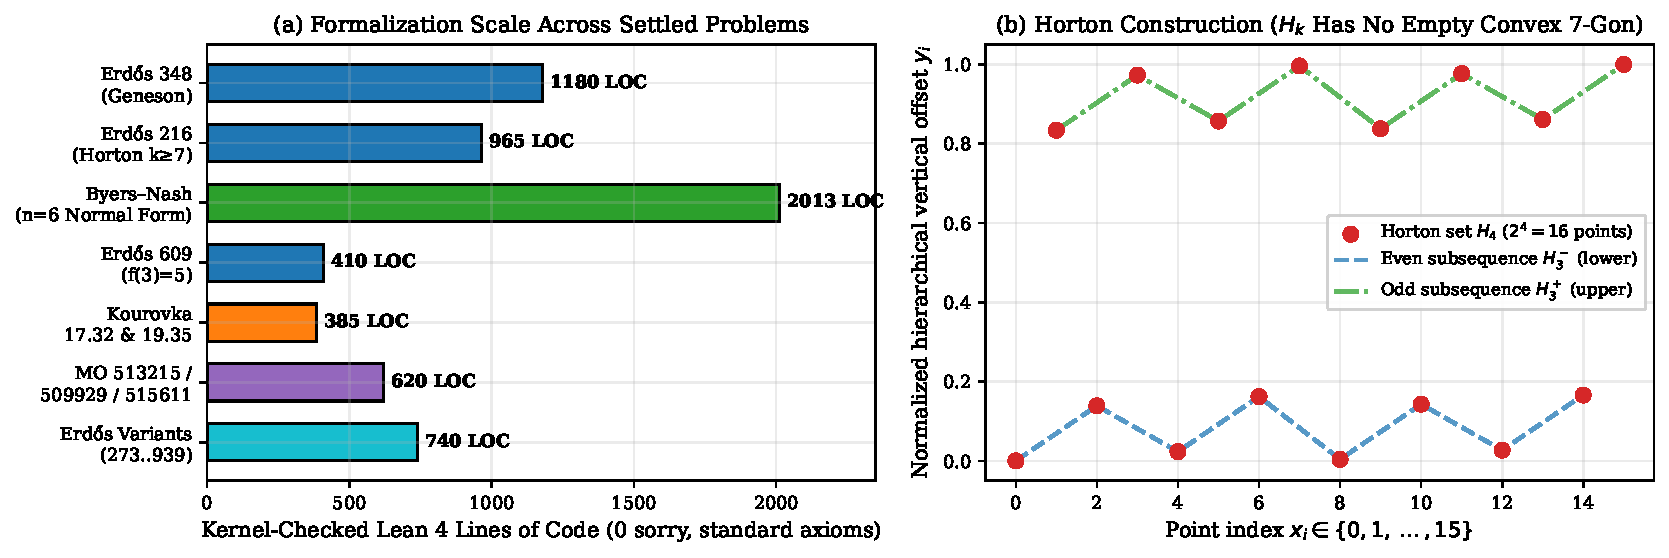
\includegraphics[width=0.96\textwidth]{figures/fig1_formalization_overview.pdf}
\caption{\textbf{Overview of the Lean~4 Formalization Suite}. (a)~Distribution of kernel-checked lines of Lean~4 code (0 \texttt{sorry}, standard axioms only) across the formalized problem packages. (b)~Visualization of the 4-level recursive Horton point set $H_4$ ($2^4 = 16$ points) formalized in \texttt{Solution.lean}, where recursive even/odd splitting with exponential vertical separation prevents any empty convex 7-gon (4-cup or 4-cap).}
\label{fig:overview}
\end{figure*}

\section{Erd\H{o}s Problem 348: Geneson's Deletion-Threshold Theorem}

Erd\H{o}s Problem~348 asks: for which integer pairs $0 \le m < n$ does there exist a non-decreasing sequence of natural numbers $a_0 \le a_1 \le a_2 \le \dots$ that is \emph{additively complete} (every sufficiently large natural number is a subset sum of distinct indices) such that:
\begin{enumerate}[leftmargin=1.4em,itemsep=1pt]
  \item deleting \emph{any} $m$ indexed terms leaves the sequence complete, but
  \item deleting \emph{any} $n$ indexed terms destroys completeness?
\end{enumerate}
Geneson~\cite{Geneson2026} recently resolved this problem completely, proving that such a sequence exists if and only if $\mathbf{m \le 1}$.

In \texttt{erdos-348-lean/Solution.lean} (1,180 lines of Lean~4), we formalize the exact \texttt{formal-conjectures} statement:
\begin{equation}
\begin{aligned}
  \bigl\{(m, n) \;\big|\; &m < n,\; \exists a\text{ monotone},\; \forall |s|=m\text{ complete},\\
  &\forall |t|=n\text{ incomplete}\bigr\}
  = \{(m, n) \mid m < n \wedge m \le 1\}.
\end{aligned}
\end{equation}

\subsection{Positive Constructions for $m = 0$ and $m = 1$}
\begin{itemize}[leftmargin=1.4em,itemsep=2pt]
  \item \textbf{Case $m = 0 < n$}: The powers of two $a_k = 2^k$ are complete (\texttt{two\_pow\_complete}: every $N \in \mathbb{N}$ has a binary representation), whereas deleting any non-empty finite set $t$ ($|t| = n \ge 1$) destroys completeness (\texttt{two\_pow\_not\_complete}: if $i \in t$, no integer $N \equiv 2^i \pmod{2^{i+1}}$ can be represented because $\sum_{j < i} 2^j = 2^i - 1 < 2^i$).
  \item \textbf{Case $m = 1 < n$}: The shifted Fibonacci sequence $a_k = F_{k+1}$ ($1, 1, 2, 3, 5, 8, \dots$) satisfies $a_k = a_{k-1} + a_{k-2}$ and Burr's sum bound $a_{k+1} \le 1 + \sum_{j < k} a_j$, so deleting any single term preserves completeness (\texttt{fibSeq\_one\_deletion}). However, deleting any $n \ge 2$ terms $i < j$ prevents representing $N = F_{m+2} - 2$ for large $m > j$ because the total sum of all non-deleted terms below $F_{m+1}$ falls strictly short of $F_{m+1} - 1$ (\texttt{fibSeq\_not\_complete}).
\end{itemize}

\subsection{Impossibility for $m \ge 2$: The Central-Interval Potential}
The core of Geneson's proof is that if $a$ remains complete after deleting \emph{any two} indices ($m \ge 2$), then for \emph{every} $n \ge 1$ there exists a finite set $t$ of size $|t| = n$ whose deletion leaves $a$ complete:
\begin{enumerate}[leftmargin=1.4em,itemsep=1pt]
  \item \textbf{2-Deletion Linear Slack Growth} (\texttt{slack\_diverges}, Lemma~3): Completeness under all 2-element deletions implies $\sum_{i < k} a_i - a_{k+1} \to \infty$ as $k \to \infty$.
  \item \textbf{Central-Interval Theorem} (\texttt{central}, Theorem~2): We formalize Geneson's discrete state transitions (\texttt{stepA}, \texttt{stepB}) and potential function (\texttt{Lemmas 6--8}) proving that once prefix slack is sufficiently large, subset sums cover a contiguous central interval $[L_k, R_k]$ whose width exceeds $a_{k+1}$.
  \item \textbf{Inductive Extension of Complete Deletions} (\texttt{extend\_core}, \texttt{exists\_complete\_deletion}, Lemma~4 \& Proposition~5): Any finite deletion $t$ preserving completeness can be augmented by a sufficiently large index $M \notin t$ ($t' = t \cup \{M\}$) while preserving completeness, inductively yielding a complete deletion of size $n$.
\end{enumerate}

\section{Erd\H{o}s Problem 216 ($k \ge 7$): Horton's Empty Convex $k$-Gon Theorem}

Erd\H{o}s Problem~216 asks whether for every $k$ there exists $g(k)$ such that any planar point set in general position of size $\ge g(k)$ contains an empty convex $k$-gon (a convex $k$-gon with no point of the set in its interior). Horton~\cite{Horton1983} famously disproved this for all $k \ge 7$.

In \texttt{lean-erdos-proofs/Solution.lean} (965 lines), we formalize Horton's theorem in both Euclidean $\mathbb{R}^2$ and the \texttt{formal-conjectures} affine-independence formulation (\texttt{Horton.erdos\_216\_ge\_seven} and \texttt{Horton.erdos\_216'}):
\begin{enumerate}[leftmargin=1.4em,itemsep=1pt]
  \item \textbf{Recursive Horton Construction}: We define the finite point sets $H_m \subset \mathbb{R}^2$ of size $2^m$ with $x$-coordinates $0, 1, \dots, 2^m - 1$ and hierarchical vertical offsets separating the even subsequence $H_{m-1}^-$ and odd subsequence $H_{m-1}^+$ by an exponential vertical gap (Figure~\ref{fig:overview}b).
  \item \textbf{Exclusion of Open 4-Cups and 4-Caps}: We prove that any convex polygon in $H_m$ whose interior is empty of points of $H_m$ decomposes into an upper chain (cap) and lower chain (cup) where neither chain can contain 4 vertices from a single layer without trapping an interleaved point of the opposite layer in its interior.
  \item \textbf{Cardinality Bound $\le 6$}: By pigeonhole across the upper/lower decomposition, every empty convex polygon in $H_m$ has at most $6$ vertices, proving $\texttt{cardSet' } k = \emptyset$ for all $k \ge 7$.
\end{enumerate}

\section{Ramsey Theory, Kourovka Counterexamples, and Erd\H{o}s Variants}

Table~\ref{tab:roster} summarizes the remaining kernel-checked theorems across \texttt{lean-erdos-proofs} and \texttt{ctrl/lean/ErdosLab}.

\begin{table}[h!]
\centering
\footnotesize
\renewcommand{\arraystretch}{1.15}
\begin{tabular}{@{}p{2.3cm}p{2.6cm}p{2.8cm}@{}}
\toprule
\textbf{Problem} & \textbf{Lean Module} & \textbf{Verified Theorem} \\
\midrule
Erd\H{o}s 609 ($n=3$) & \texttt{Erdos609.lean} & $f(3)=5$ on 3-colored $K_9$ (Cai 2026) \\
Kourovka 17.32 & \texttt{Kourovka17\_32.lean} & Free-group Cayley--Hamilton fails at $n=2$ \\
Kourovka 19.35 & \texttt{Kourovka19\_35.lean} & $A_4$ has no $(2,3,2)$ subset factorization \\
MO 513215 & \texttt{MO513215.lean} & $a_n = \frac{n(n+3)}{2} \Rightarrow S(0)=\frac{11}{9}, S(1)=1$ \\
MO 509929 & \texttt{SquareGraphDiameter.lean} & Square-product graph on $\mathbb{N}^+$ has diameter 3 \\
MO 515611 & \texttt{FerrisWheel.lean} & $907200$ is a Ferris wheel number (order 210) \\
MO 501066 & \texttt{LcmHighlyAbundant.lean} & $\mathrm{lcm}(1\dots 200000)$ is not highly abundant \\
Erd\H{o}s 273 ($p \ge 3$) & \texttt{ErdosLab/Erdos273.lean} & 12-modulus strict covering mod 720 \\
Erd\H{o}s 292 ($\ge 2$) & \texttt{ErdosLab/Erdos292.lean} & $\mathbb{N}\setminus A$ finite via $\{2,3,6\}$ \& $\{2,4,6,12\}$ \\
Erd\H{o}s 318 (even) & \texttt{ErdosLab/Erdos318.lean} & Shifted odd-square binary block $f$ with $0 \notin \text{range}$ \\
Erd\H{o}s 834 (3-unif.) & \texttt{ErdosLab/Erdos834.lean} & 7-vertex, 9-edge criticality witness \\
Erd\H{o}s 885 ($k=3$) & \texttt{ErdosLab/Erdos885.lean} & $\{120,208,672\}$ share $d \in \{2,14,22\}$ \\
Erd\H{o}s 939 ($r=6$) & \texttt{ErdosLab/Erdos939.lean} & Infinite coprime 6-powerful triples $t = 6k+1$ \\
\bottomrule
\end{tabular}
\caption{Kernel-checked combinatorics, algebra, and number-theory formalizations.}
\label{tab:roster}
\end{table}

\begin{thebibliography}{9}
\small
\bibitem{FormalConjectures}
The Formal Conjectures Authors, ``\texttt{formal-conjectures}: A collection of formalized statements of conjectures in Lean~4,'' GitHub repository, 2025--2026.
\bibitem{Geneson2026}
J.~Geneson, ``Deletion thresholds and exponential examples for complete sequences,'' \texttt{arXiv:2609.25107}, 2026.
\bibitem{Horton1983}
J.~D.~Horton, ``Sets with no empty convex 7-gons,'' \emph{Canadian Mathematical Bulletin}, vol.~26, no.~4, pp.~482--484, 1983.
\end{thebibliography}

\end{document}
